
Se desea trabajar con series temporales sobre mediciones climatológicas. 
En concreto, se eligen las variables de temperatura del aire, humedad relativa y presión atmosférica en la superficie.
Dichas variables son estudiadas con frecuencia horaria, en el intervalo comprendido entre el 1 de marzo de 2023 y el 28 de febrero de 2025.

Es relevante el uso de datos en un período múltiplo del año, para asegurar que se capturan las variaciones estacionales y que el conjunto de datos está suficientemente equilibrado.

\section{Fuentes de los datos}

Se han empleado 2 fuentes para recopilar las mediciones: 
\begin{itemize}
    \item \textbf{Grafcan}: Cartográfica de Canarias, S.A. es una empresa pública de la Comunidad Autónoma de Canarias. Dispone de una red de estaciones meteorológicas cuyas
    mediciones son accesibles mediante una API REST de acceso gratuito previa solicitud de una clave\cite{grafcan_sensores}. 
    \item \textbf{Open-Meteo}: API pública de código abierto que proporciona datos de múltiples proveedores de meteorología. Este servicio no dispone de estaciones de medición
    propias, sino que recopila pronósticos de diferentes modelos de predicción climatológica. 

    Se emplea la API de predicciones pasadas\cite{open_meteo_api}. Se seleccionan los modelos ICON Global del servicio meteorológico alemán (DWD) y el modelo ARPEGE Europe de Météo-France. Ambos modelos se actualizan cada 3 horas. 
    Se explora la posibilidad de emplear as predicciones del modelo HAROME de la AEMET, pero no están disponibles de forma pública
\end{itemize}

Se eligen 4 ubicaciones de la isla de Tenerife con distintas características climáticas para el conjunto de entrenamiento y evaluación:
\begin{itemize}
    \item \textbf{San Cristóbal de La Laguna 1}: La Cuesta, 35 metros de altitud.
    \item \textbf{San Cristóbal de La Laguna 2}: La Punta del Hidalgo, 54m.
    \item \textbf{La Orotava}: Camino de Chasna, 812m.
    \item \textbf{Arona}: Punta de Rasca, 25m.
\end{itemize}

Así mismo, se escogen 2 ubicaciones para el conjunto de test, nunca vistas en el ajuste del modelo:
\begin{itemize}
    \item \textbf{Garachico}: La Montañeta, 922 m.
    \item \textbf{Santa Cruz de Tenerife}: Polígono Costa Sur, 92m.
\end{itemize}

Las ubicaciones han sido elegidas al contar con estaciones de medición de Grafcan.
Sus posiciones se muestran en la Figura \ref{mapa_estaciones}, señaladas en rojo. De izquierda a derecha: Arona, La Orotava y San Cristóbal de La Laguna.

\begin{figure}[htb]
   \centering
   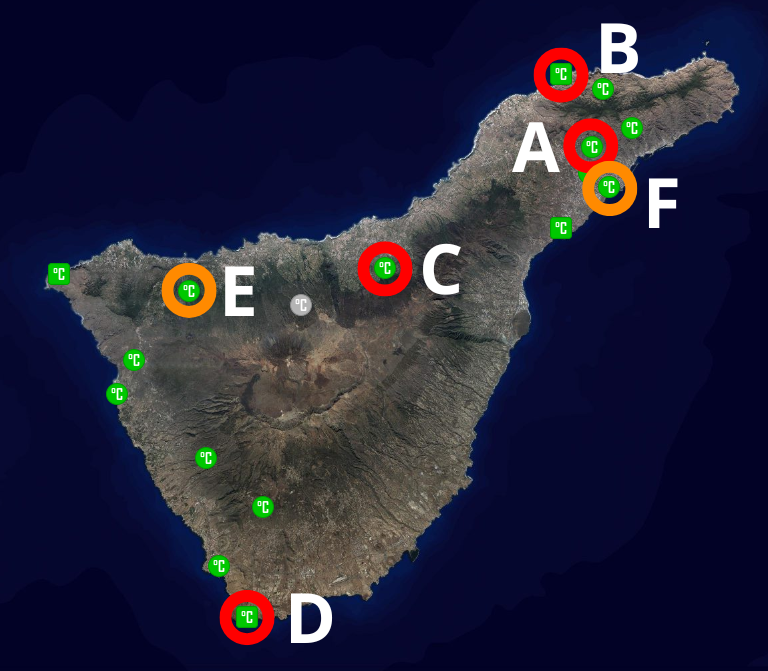
\includegraphics[width=0.6\linewidth]{images/mapa_estaciones}
   \caption{Mapa de las estaciones climatológicas Grafcan empleadas.}
   \label{mapa_estaciones}
\end{figure}

Inicialmente se valoró emplear las estaciones correspondientes a Los Cristianos, Santiago del Teide o la Punta de Teno, pero fueron descartadas por dos motivos: 
se detectó que existían períodos prolongados con datos faltantes en las mediciones de Grafcan. Algunas de ellas también exhibían poca correlación entre las mediciones
del servicio Grafcan y las de Open-Meteo, lo que podría afectar la calidad de los datos.

\bigskip

\section{Proceso de adquisición y almacenamiento}

Para automatizar la adquisición de datos, se emplea la herramienta de orquestación node-red, que permite crear flujos de información mediante nodos que realizan tareas específicas o ejecutan códgio de JavaScript.
En dicha herramienta se desarrollan dos paneles, uno para cada fuente de datos. 
Así mismo, dentro de cada panel se desarrollan dos flujos, uno para la adquisición de datos en un intervalo dado, y otro para la adquisición de datos en tiempo real, en particular, 
se establece la recogida de datos cada 6 horas.

\subsection{Flujos de adquisición de Grafcan}
Debido al funcionamiento de la API de Grafcan, se debe realizar una llamada para obtener la serie temporal de cada variable meteorológica de cada estación.
Posteriormente, se unen las series de cada estación en una única serie, que se almacena en una base de datos PostgreSQL. Este flujo está reflejado en la figura \ref{grafcan_flows}.
\begin{figure}[htb]
   \centering
   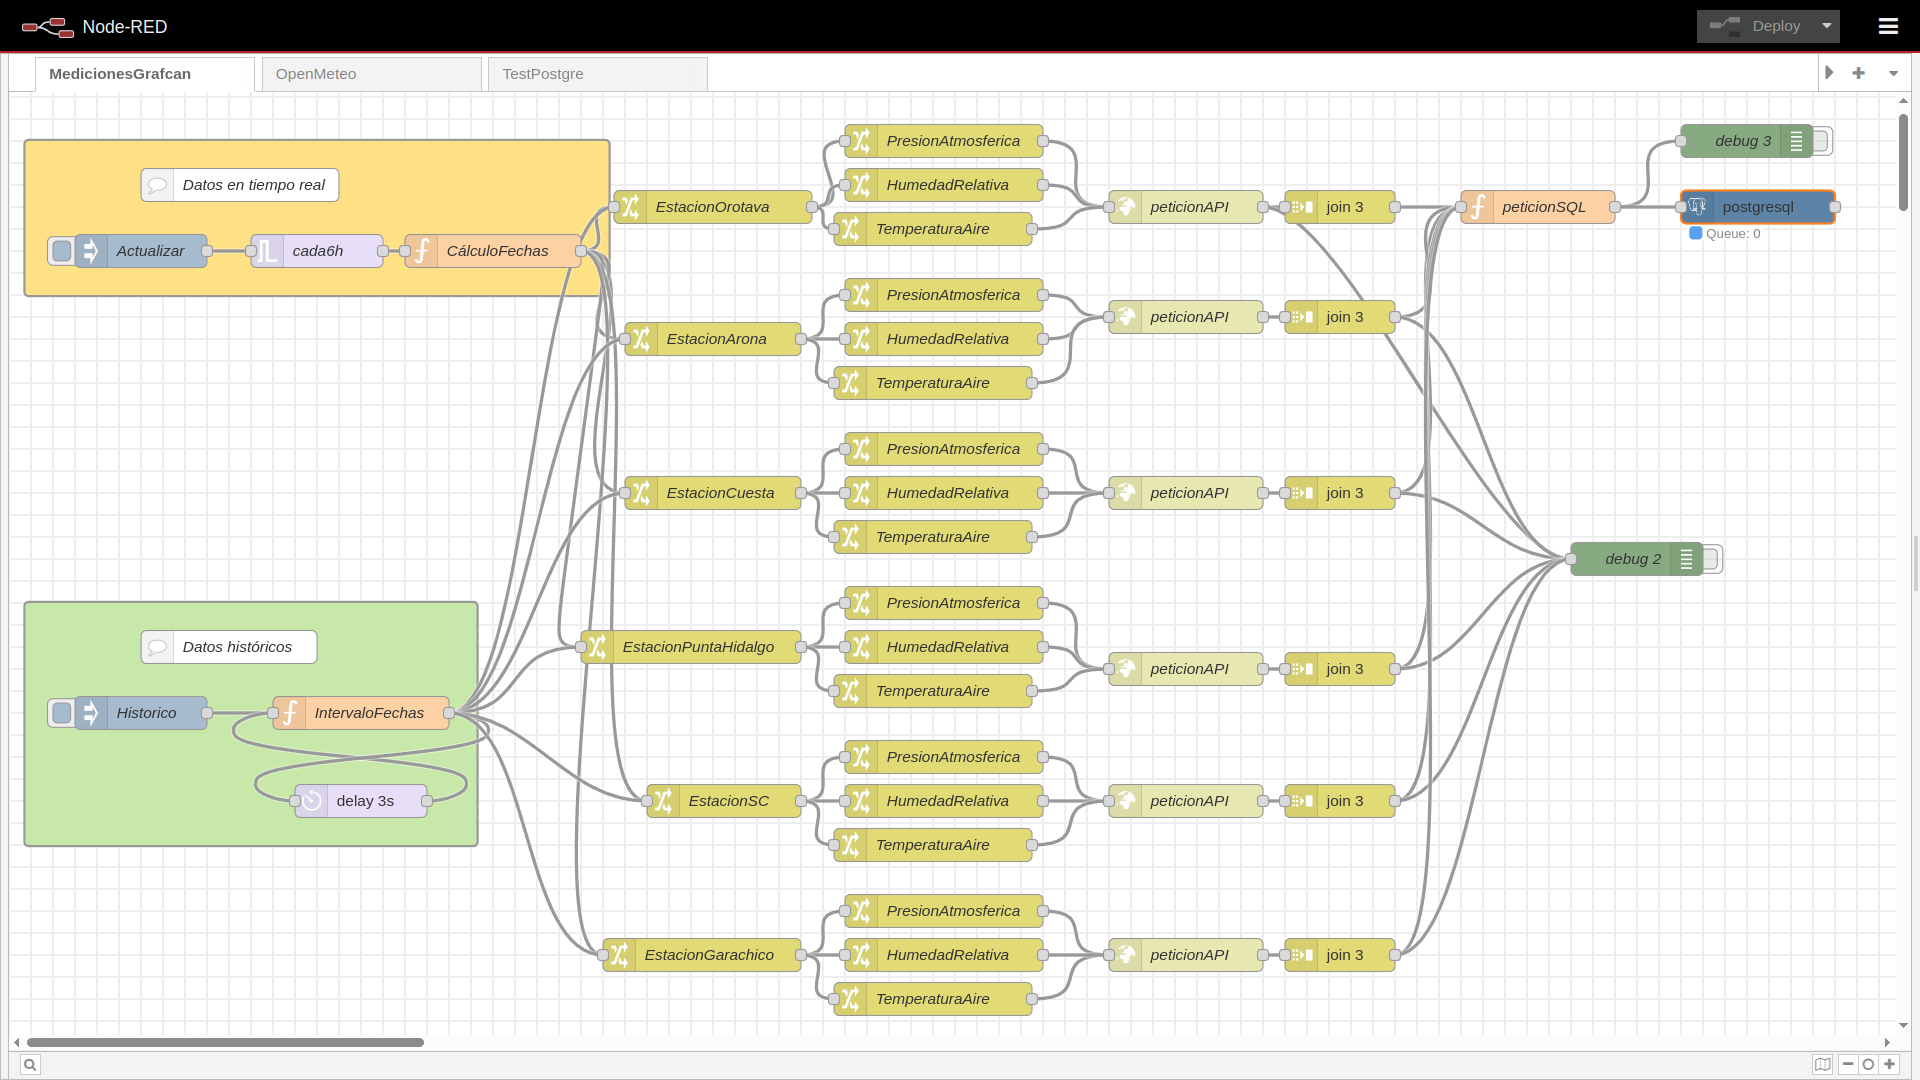
\includegraphics[width=1\linewidth]{images/node-red_grafcan.png}
   \caption{Flujo de adquisición de datos de Grafcan en node-red.}
   \label{grafcan_flows}
\end{figure}

Las mediciones de Grafcan se recogen apróximamente cada 10 minutos, si bien la frecuencia no es consistente y en ocasiones es mayor. Para manejar esta variabilidad, 
en este nivel los datos se agregan cada 10 minutos, usando la media de las mediciones del intervalo.

\subsection{Flujos de adquisición de Open-Meteo}
Existe una rama para obtener los datos del modelo ICON y otra para el modelo ARPEGE. Se establecen las coordenadas de cada ubicación como las de la estación de Grafcan seleccionada 
y se realiza una llamada a la API por cada localización y cada modelo, como se observa en la figura \ref{open-meteo_flows}. 
Los resultados se almacenan en una base de datos PostgreSQL.
\begin{figure}[htb]
   \centering
   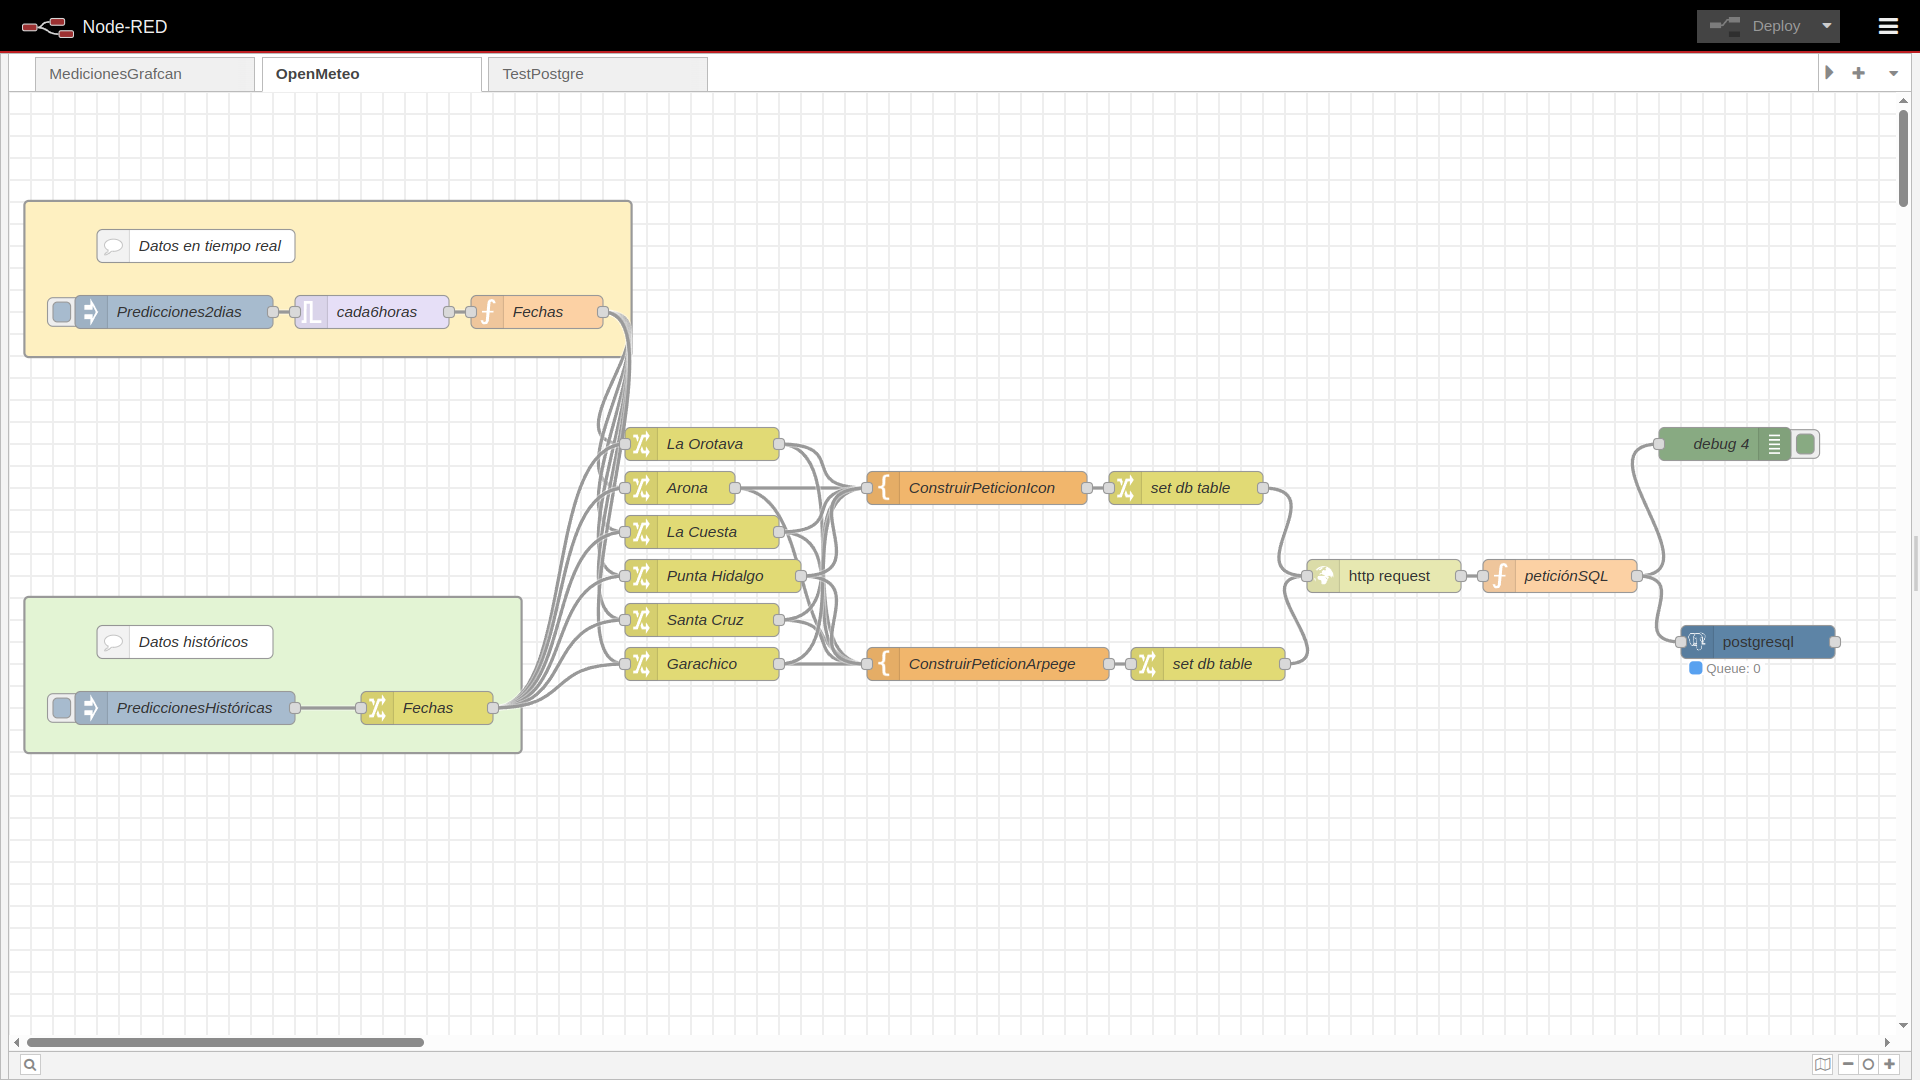
\includegraphics[width=1\linewidth]{images/node-red_open-meteo.png}
   \caption{Flujo de adquisición de datos de Open-Meteo en node-red.}
   \label{open-meteo_flows}
\end{figure}

\subsection{Almacenamiento}
Se estudian distintas alternativas para el almacenamiento de los datos.
Se opta por emplear TimescaleDB, una extensión del popular sistema PostgreSQL
de bases de datos relacionales, especialmente adaptada para el manejo de series temporales. 

Se establece un servidor TimescaleDB en un contenedor Docker. Se configura una tabla para cada estación y cada fuente: Grafcan, Open-Meteo ICON y Open-Meteo ARPEGE. 
Cada tabla emplea como índice y clave primaria la fecha y hora de la medición, así como su zona horaria. Las otras columnas se corresponden a la temperatura media del aire
 en grados Celsius, la humedad relativa en porcentaje y la presión atmosférica en superficie medida en hPa.

Es importante señalar que las mediciones de Grafcan y Open-Meteo codifican las horas en UTC, en vez de la hora local, puesto que UTC es independiente a los cambios de horario
y de esta forma se mantiene la consistencia de los datos.

\section{Preprocesado}

Se desarrolla un cuaderno de Jupyter para realizar el preprocesado de los datos. Este proceso se aplica para cada estación.

En primer lugar, se obtienen las series temporales de las 3 fuentes, Grafcan y los dos modelos de Open-Meteo, para el período entre el 1 de marzo de 2023 y el 28 de febrero de 2025.
Se agregan los datos con frecuencia horaria mediante la media. 

\textbf{Nota:} En la estación de Garachico, usada para el test, el período empleado es del 1 de marzo de 2024 al 28 de febrero de 2025, puesto que el período de 2023 tiene 
un gran número de datos faltantes.

\subsection{Visualización}
Se visualizan los datos de cada variable para cada año. Podemos ver ejemplos en las figuras \ref{visualizacion_1}, \ref{visualizacion_2} y \ref{visualizacion_3}.

Se observa claramente que en la presión atmosférica las mediciones de todas las fuentes son muy similares. Sin embargo, 
en la temperatura del aire y la humedad relativa se aprecian diferencias entre las distintas fuentes.
\begin{figure}
    \centering
    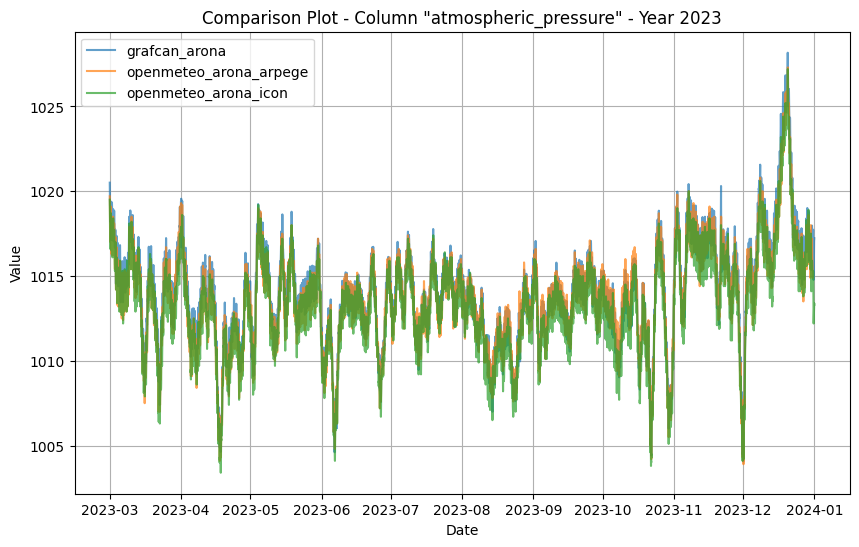
\includegraphics[width=.8\linewidth]{images/visualizacion_1.png}
    \caption{Visualización de la presión atmosférica en Arona durante 2023.}
    \label{visualizacion_1}
\end{figure}
\begin{figure}
    \centering
    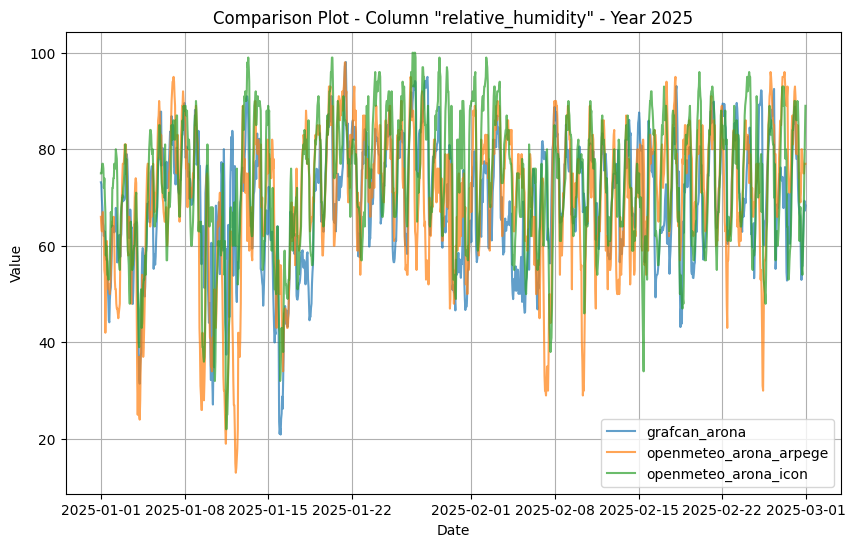
\includegraphics[width=.8\linewidth]{images/visualizacion_2.png}
    \caption{Visualización de la temperatura del aire en Arona durante 2024.}
    \label{visualizacion_2}
\end{figure}
\begin{figure}
    \centering
    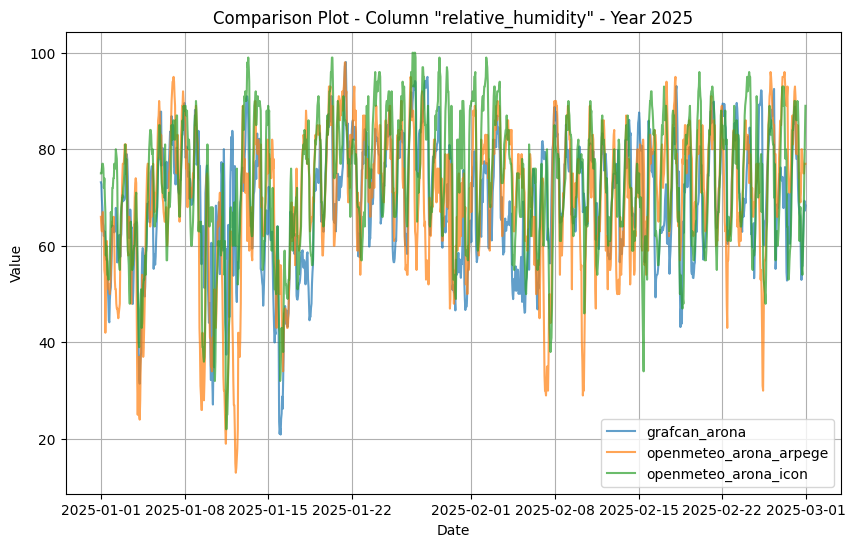
\includegraphics[width=.8\linewidth]{images/visualizacion_3.png}
    \caption{Visualización de la humedad relativa en Arona durante 2025.}
    \label{visualizacion_3}
\end{figure}

Cabe destacar que en la variable de humedad relativa se observa una gran variabilidad entre los datos de las distintas fuentes, lo que puede ser ??????

\subsection{Manejo de datos faltantes}
Se detectan los datos faltantes para cada fuente. Las estadísticas se muestran en la tabla \ref{tabla_datos_faltantes}.
\begin{table}[htb]
    \centering
    \begin{tabular}{|c|c|c|c|}
        \hline
        Estación & Grafcan & Open-Meteo ICON & Open-Meteo ARPEGE \\
        \hline
        La Laguna 1 (La Cuesta) & 0.2\% & 0.1\% & 0.1\% \\
        La Laguna 2(La Punta del Hidalgo) & 0.3\% & 0.2\% & 0.2\% \\
        La Orotava & 0.5\% & 0.4\% & 0.4\% \\
        Arona & 17 & 0 & 35 \\
        Garachico & 5 & 0 & 0 \\
        Santa Cruz de Tenerife & 0.5\% & 0.4\% & 0.4\% \\
        \hline
    \end{tabular}
    \caption{Datos faltantes por estación y fuente de datos (en horas)}
    \label{tabla_datos_faltantes} 
\end{table}

